\section{Extract unit cell protocol}
\label{app:extractUnitCell}%a070
Protocol designed to obtain the smallest asymmetric subunit of an electron density map having certain types of rotational symmetry.\\
WARNING: This protocol requires the starting volume located in the center of coordinate axes.\\

\begin{itemize}
  \item \scipion menu:\\
  \ttt{Protocols SPA -> Model building} (\ffigure{fig:app_protocol_extractUnitCell_1} (A))\\
  
  \item Protocol form parameters (\ffigure{fig:app_protocol_extractUnitCell_1} (B)):\\
  
  \begin{figure}[H]
    \centering 
    \captionsetup{width=.7\linewidth} 
    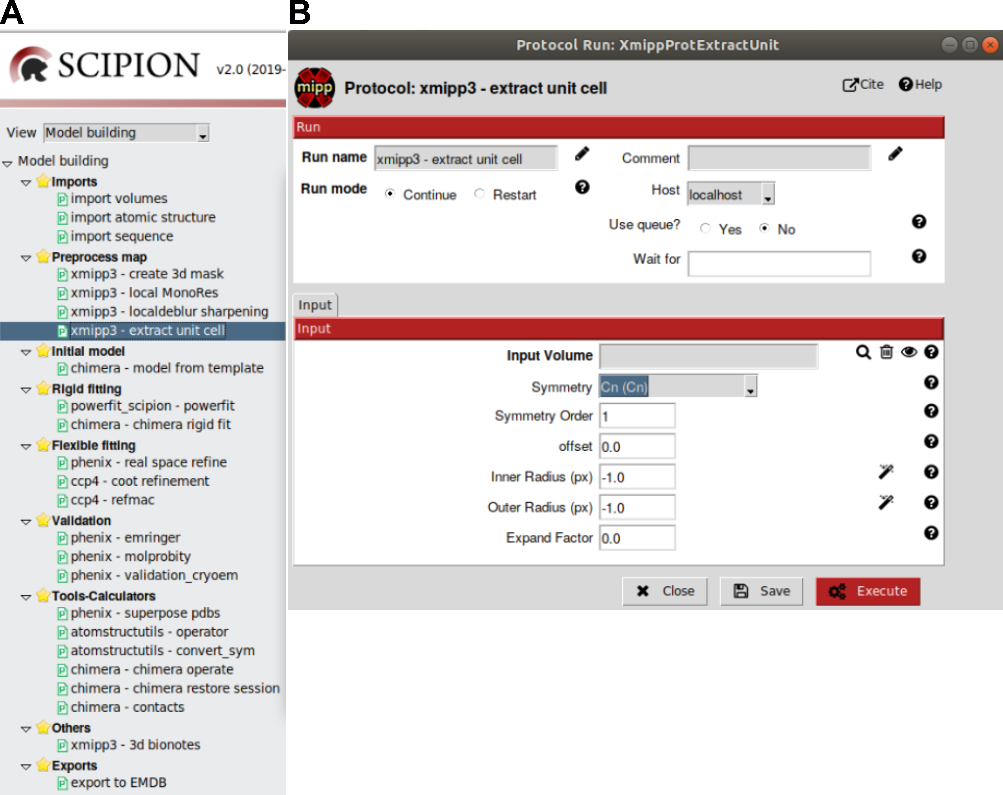
\includegraphics[width=0.90\textwidth]{Images_appendix/Fig107.pdf}
    \caption{Protocol \scommand{extract unit cell}. A: Protocol location in \scipion menu. B: Protocol form.}
    \label{fig:app_protocol_extractUnitCell_1}
   \end{figure}
  
  \begin{itemize}
  \item \ttt{Input Volume}: Volume already downloaded in \scipion from which the unit cell will be extracted.\\
  \item \ttt{Symmetry}: In this protocol, symmetry refers only to rotational symmetry, also known in biology as radial symmetry. This symmetry is the property of volumes to preserve their shape after a partial turn around a symmetry axis.  \\
  Types of rotational symmetry included in this protocol are shown in \ffigure{fig:app_protocol_extractUnitCell_2}. Two names appear in each case, the first one corresponds to \ttt{XMIPP} nomenclature of symmetry because we are using \ttt{XMIPP} package, and the second one (in brackets) follows the general \scipion nomenclature. Current \scipion nomenclature is $Chimera$'s nomenclature, which is, in turn, the same symmetry nomenclature of the International Union of Cristallography. \\
  
    \begin{figure}[H]
    \centering 
    \captionsetup{width=.7\linewidth} 
    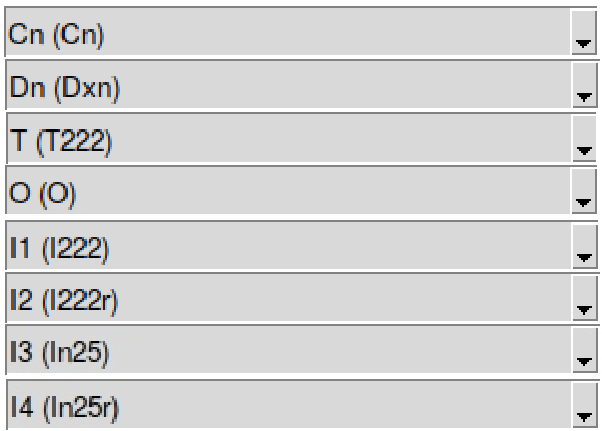
\includegraphics[width=0.25\textwidth]{Images_appendix/Fig108.pdf}
    \caption{Protocol \scommand{extract unit cell}. Types of rotational symmetry.}
    \label{fig:app_protocol_extractUnitCell_2}
   \end{figure}
   
  \begin{itemize}
  \item Cyclic symmetry \ttt{Cn (Cn)}: Only one symmetry axis goes through the geometric center of the volume. Two more form parameters are shown when this type of symmetry is selected:\\
   \begin{itemize}
    \item \ttt{Symmetry Order}: Number of times (\ttt{n}) in which a volume shows the same shape when the volume rotates around the symmetry axis from 0 to 360º. If the same shape is only obtained after turning 360º, \ttt{n = 1}, which means that the volume has no symmetry. \ttt{360º/n} determines the rotation angle. \\ 
	\item \ttt{offset}: Starting angle around Z axis.\\ 
   \end{itemize}
  \item Dihedral symmetry \ttt{Dn (Dn)}: Two perpendicular symmetry axis go through the geometric center of the volume. As in the case of cyclic symmetry, two more form parameters are shown when this type of symmetry is selected:\\
   \begin{itemize}
    \item \ttt{Symmetry Order}: Number of times (\ttt{n}) in which a volume shows the same shape when the volume rotates around both symmetry axes from 0 to 360º. Analogously, \ttt{360º/n} determines the rotation angle.\\ 
	\item \ttt{offset}: Starting angle around Z axis.\\ 
   \end{itemize}
  \item Tetrahedral symmetry \ttt{T (T)}: Four symmetry axes go from each vertex to the opposing face center (order 3), and three symmetry axes join opposing edges (order 2). \ttt{Symmetry order = 12}.\\
  \item Octahedral symmetry \ttt{O (O)}: Three symmetry axes join opposing vertices (order 4), four symmetry axes join opposing face centers (order 3), and six symmetry axes join opposing edges (order 2). \ttt{Symmetry order = 24}.\\
  \item Icosahedral symmetries \ttt{I1 (I222), I2 (I222r), I3 (In25), I4 (In25r)}: Six symmetry axes join opposing vertices (order 5), 10 symmetry axes join baricenters of opposing faces (order 3), and 15 symmetry axes join opposing edges (order 2). \ttt{Symmetry order = 60}. Each type of icosaedral symmetry depends on its initial orientation. Check in \chimera each one of them from the main graphics menu: \ttt{Tools -> Higher-Order Structure -> Icosahedron Surface -> Orientation} (\ttt{I222}: order 2 axes follow XYZ coordinate axes; \ttt{I222r}: idem rotated 90º around Z axis; \ttt{In25}: an order 2 axis and an order 5 axis follow Y and Z axes, respectively, \ttt{In25r}: idem rotated 90º around Z axis.\\
  \end{itemize}
  
  \item \ttt{Inner Radius (px)}: Minimal distance from the geometric center that delimits inwards the part of the map electron density that will be included in the extracted volume. A wizard symbol on the right side of this parameter can be helpful to select this radius.\\
  \item \ttt{Outer Radius (px)}: Maximal distance from the geometric center that delimits outwards the part of the map electron density to be included in the extracted volume. Again, the wizard symbol on the right side of this parameter can be helpful to select this radius.\\
  \item \ttt{Expand Factor}: Additional fraction of the asymmetrical unit cell that will be included in the extracted volume.\\
  \end{itemize}

  \item Protocol execution:\\
  
  Press the \ttt{Execute} red button at the form bottom.\\
  Adding specific extracted volume label is recommended in \ttt{Run name} section, at the form top. To add the label, open the protocol form, press the pencil symbol at the right side of \ttt{Run name} box, complete the label in the new opened window, press OK, and finally close the protocol. If you want to run again this protocol, do not forget set to \ttt{Restart} the \ttt{Run mode}.\\
  
  \item Visualization of protocol results:\\
  
  After executing the protocol, press \ttt{Analyze Results} and a small window will be opened (\ffigure{fig:app_protocol_volume_2}). This window allows you to select between \ttt{chimera} ($Chimera$ graphics window) and \ttt{slices} ($ShowJ$, the default \scipion viewer), to visualize the volume.
  
    \begin{figure}[H]
    \centering 
    \captionsetup{width=.7\linewidth} 
    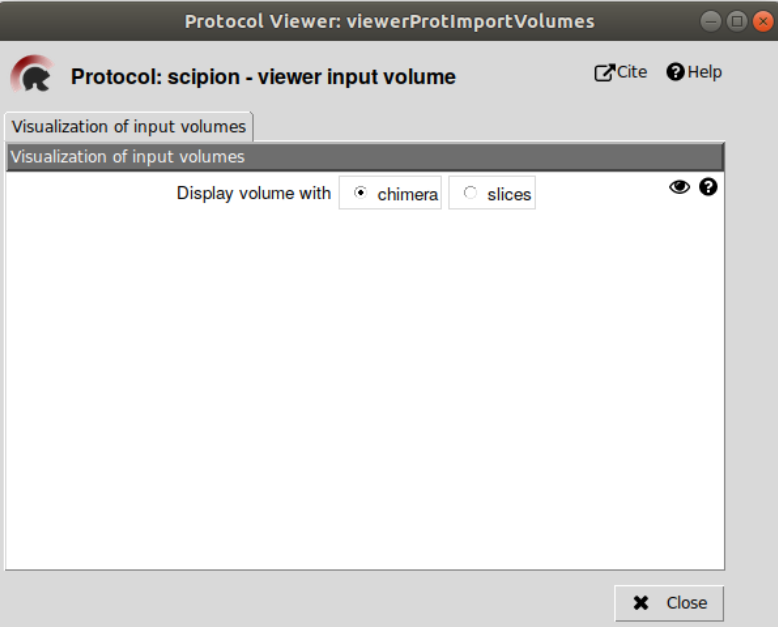
\includegraphics[width=0.70\textwidth]{Images_appendix/Fig101.pdf}
    \caption{Menu to select a visualization tool.}
    \label{fig:app_protocol_volume_2}
   \end{figure}
   
   \begin{itemize}
   \item \ttt{chimera}: $Chimera$ graphics window\\
   
   Initial whole volume and extracted volume appear referred to the origin of coordinates in \chimera. To show the relative position of the volume, the three coordinate axes are represented; X axis (red), Y axis (yellow), and Z axis (blue) (\ffigure{fig:app_protocol_volume_3}). Coordinate axes, initial volume, and extracted unit cell volume are model numbers \ttt{\#0}, \ttt{\#1} and \ttt{\#2}, respectively, in $Chimera$ \ttt{Model Panel}. Volume coordinates and pixel size can be checked in $Chimera$ main menu \ttt{Tools -> Volume Data -> Volume Viewer -> Features -> Coordinates: Origin index/ Voxel size}. Take into account that coordinates appear in pixels while they have been introduced in \AA.\\
   
  \item \ttt{slices}: $ShowJ$\\
   
   \url{https://github.com/I2PC/scipion/wiki/ShowJ}\\
   Each volume can be independently visualized by selecting it in the upper menu as arrow indicates in \ffigure{fig:app_protocol_extractUnitCell_3}.
   
   \begin{figure}[H]
    \centering 
    \captionsetup{width=.7\linewidth} 
    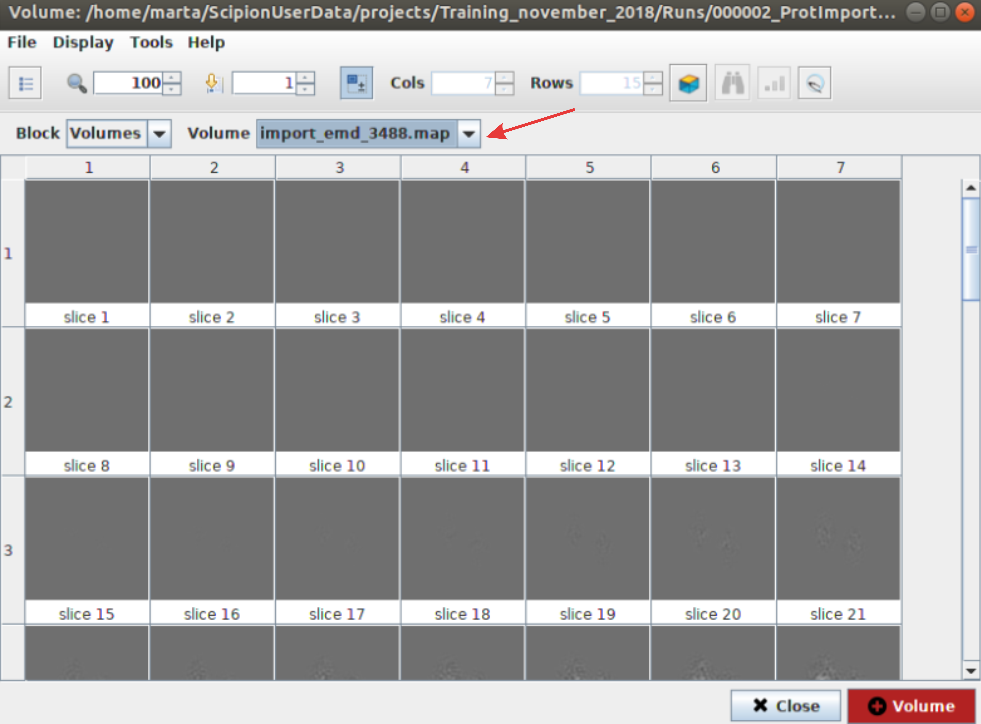
\includegraphics[width=0.75\textwidth]{Images_appendix/Fig109.pdf}
    \caption{Protocol \scommand{extract unit cell}. Volume selection with ShowJ.}
    \label{fig:app_protocol_extractUnitCell_3}
   \end{figure}
   
   \end{itemize}

 \item Summary content:\\
  \begin{itemize}
     \item Protocol output (below \scipion framework):\\ \ttt{xmipp3 - extract unit cell -> ouputVolume}; Volume (x, y, and z dimensions, sampling rate).\\
     \item \ttt{SUMMARY} box:\\ Empty\\
    \end{itemize}

  \end{itemize}
